\chapter{Closing Remarks}
\label{cha:ClosingRemarks}

\section{Criticism}

The previous chapters addressed the advantages, benefits and possibilities of decentralized finance. But as always, there is no free lunch.
Even decentralized finance is not immune against criticism. This section provides a brief overview of a few of the most relevant issues coming
from detractors as well of a data-based evaluation whether they are valid or not.

Cryptocurrencies like Bitcoin that are using a proof-of-work algorithmn in order to achieve consensus have an extremely high power consumption.
Figure \ref{fig:BtcEnergy} shows that the Bitcoin network alone has a yearly electrical energy use of 77.78 TWh, just passing Austria with
74.1 TWh in October 2020. While this are numbers, that cannot be blandished, it is important to keep in mind that the mining algorithm on
Bitcoin is jointly responsible for its high value and is vital for the network, in order to operate in a proper and secure way.

A solution would be a proof-of-stake algorithm which is the choice of the majority of newer coins. Ethereum is already moving to proof-of-stake
as part of its update Ethereum 2.0 but that is not happening on Bitcoin anytime soon. At least 73\% of Bitcoin's electricity comes from
renewable energy sources, as investigated by researches from CoinShares \cite[p.\ 8]{CoinShares2019}. This has economical reasons. In an open
market economy, Bitcoin miners will always move to those places where energy is cheaper than anywhere else. The majority of Bitcoin mining is
done in Sichuan, China because the hydroelectrcity is very cheap in the rainy season. But there are also other attractive locations such as
Iceland and its eco-friendly geothermal energy sources.

\begin{figure}
\centering
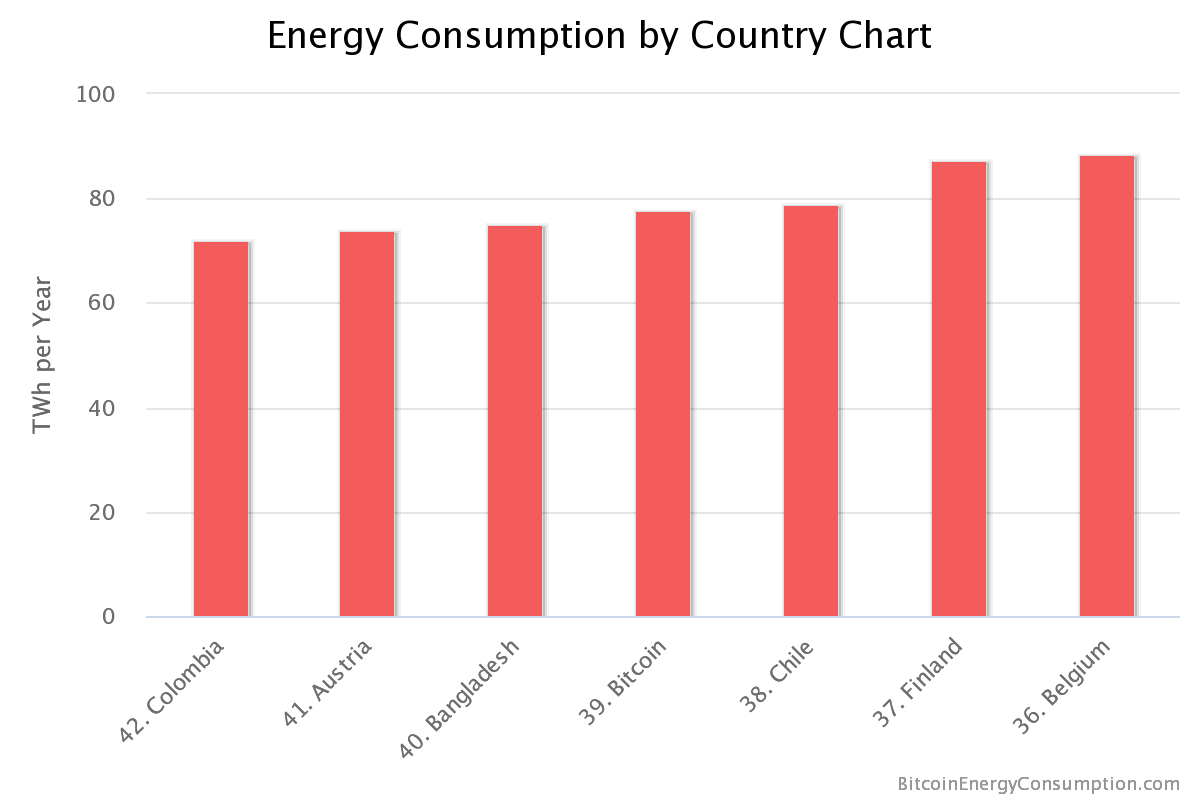
\includegraphics[width=.95\textwidth]{energy-consumption-by-co}
\caption{Bitcoin's Energy Consumption Compared to Countries \cite{Digiconomist2020}.}
\label{fig:BtcEnergy}
\end{figure}

Another popular objection is the high use of cryptocurrencies for criminalism and money laundering. While there is obviously no data about the
actual numbers of value used illegally, the majority of illicit assets still take place in fiat currencies. It is only logical, that
cryptocurrencies are the preferred choice to be used on darknet markets. But that is not a problem of the crypocurrencies themselves, as like any
technology, they are just tools which can help to achieve either good or bad things. Shifting the focus back to decentralized finance in particular,
the number of illegal activities is plummeting, as there are even more privacy focused coins like Zcash, Monero and Dash \cite[p.\ 13]{FDD2018}.

As of the arise of a lot new projects in the area of decentralized finance, some of them are exposed to ponzi schemes and similar frauds, as
fairly new projects usually are very centralized and only dispense control after time. There is no real solution for that, except enouraging
people to do their own research beforehand and by following the principle of only investing in what you understand. But even if the founders
have no bad intentions, it is still possible that users loose money due to errors in the code. This is specifically a real problem on
Ethereum, as of its turing completeness increases the risk of unconciously adding bugs to the code. DeFiChain \cite{DeFiChain}, 
a Bitcoin fork specifically adapted for decentralized financial use cases, tries to solve that problem by restricting the interaction with the
blockchain by only using few commands.

* code errors
* ponzi schemes

\section{Risks}
---0.5 pages---
* smart contract risk
* volatility
* regulation: central interfaces
* black swans
* scams
* hacks
* only things happen on DeFi that harm people (betting on death)

\section{Prospective Impact}
--- 0.5 pages ---